\documentclass[TIDYMASTER.tex]{subfiles} 
\begin{document} 

%=============================================================================== %
\begin{frame}[fragile]
	\frametitle{Tidy Data with \texttt{R}}
	\Large
\begin{figure}
\centering

\includegraphics[width=0.7\linewidth]{Rstudio}
\end{figure}
%	© Garrett Grolemund. Pre-order Data Science with R at shop.oreilly.com
\begin{itemize}
\item \textit{Data Science with R} by Garrett Grolemund
\item Chapter: Data Tidying
\end{itemize}	


\end{frame}

%=============================================================================== %
\begin{frame}
	\frametitle{Tidy Data with \texttt{R}}
	\Large
	\noindent \textbf{DSR Example Data Sets}
	\begin{itemize}
		%\item You can organize tabular data in many ways. For example, 
		\item The data sets in the DSR Package show the same data, but  organized in four entirely different ways. 
		\item Each data set shows the same values of four variables country, year, population, and cases, but each data set organizes the values into a different layout. 
		%\item You can access the data sets in the DSR package.
	\end{itemize}
	
\end{frame}
%=============================================================================== %
\begin{frame}[fragile]
	\frametitle{Tidy Data with \texttt{R}}
	\Large
	\begin{itemize}
		% \item	You will also need to install the tidyr, devtools, and DSR packages. 
		% \item To install, tidyr and devtools, open RStudio and run the command
		% \item DSR is a collection of data sets assembled for this book and saved online as a github repository (github.com/garrettgman/DSR).
		\item To install DSR, run the command
	\end{itemize}
	{
		\large
	\begin{framed}
		\begin{verbatim}
		install.packages(c("tidyr", "devtools"))
		
		devtools::install_github("garrettgman/DSR")
		\end{verbatim}
	\end{framed}
}
	
	
\end{frame}
%%=============================================================================== %
%\begin{frame}
%	\frametitle{Tidy Data with \texttt{R}}
%	\Large
%\begin{itemize}
%%\item In the wild, data sets come in many different formats, but each computer program expects your data to be organized in a predetermined way, which may vary from program to program.
%%\item In this chapter, you will learn the best way to organize your data for R, a task that I call data tidying. 
%%\item This may seem like an odd place to start, but 
%\item Tidying data is the most fruitful skill you can learn as a data scientist. It will save you hours of time and make your data much easier to visualize, manipulate, and model with R.
%\end{itemize}
%
%\end{frame}
%%=============================================================================== %
%\begin{frame}
%	\frametitle{Tidy Data with \texttt{R}}
%	\Large
%Note that this chapter explains how to change the format, or layout, of tabular data. To learn how to use different file formats with R, see Appendix B: Data Sources.
%\end{frame}
%=============================================================================== %
%\begin{frame}
%	\frametitle{Tidy Data with \texttt{R}}
%	\Large
%\noindent \textbf{Outline}
%\begin{itemize}
%\item In Section 2.1, you will learn how the features of R determine the best way to layout your data. 
%\item This section introduces “tidy data,” a way to organize your data that works particularly well with R.
%\end{itemize}
%
%\end{frame}

%=============================================================================== %
%\begin{frame}
%	\frametitle{Tidy Data with \texttt{R}}
%	\Large
%Section 2.3 explains how to split apart and combine values in your data set to make them easier to access with R.
%\end{frame}


%=============================================================================== %

%=============================================================================== %
\begin{frame}[fragile]
	\frametitle{Tidy Data with \texttt{R}- Data Set 1}
	\large
\begin{framed}
\begin{verbatim}
library(DSR)
# Data set one
table1
## Source: local data frame [6 x 4]
## 
##       country year  cases population
## 1 Afghanistan 1999    745   19987071
## 2 Afghanistan 2000   2666   20595360
## 3      Brazil 1999  37737  172006362
## 4      Brazil 2000  80488  174504898
## 5       China 1999 212258 1272915272
## 6       China 2000 213766 1280428583
\end{verbatim}
\end{framed}
\end{frame}
%=============================================================================== %
\begin{frame}[fragile]
	\frametitle{Tidy Data with \texttt{R}}
	\Large
	\vspace{-1cm}
	\begin{itemize}
		\item In \texttt{table1} (previous slide), each variable is placed in its own column, each observation in its own row, and each value in its own cell.
		\item It properly complies with the \textit{Principles of Tidy Data}. \bigskip
		\item On the next set of slides - we will look at three more layouts (with the last layout comprising two separate tables)
		
%		\item Tidy data builds on a premise of data science that data sets contain both values and relationships.
%		\item  Tidy data displays the relationships in a data set as consistently as it displays the values in a data set.
	\end{itemize}
	
\end{frame}
%=============================================================================== %
\begin{frame}[fragile]
	\frametitle{Table 2 (sed)}
	\large
	\begin{framed}
		\begin{verbatim}
# Data set two
table2

## Source: local data frame [12 x 4]
## 
##        country year        key      value
## 1  Afghanistan 1999      cases        745
## 2  Afghanistan 1999 population   19987071
## 3  Afghanistan 2000      cases       2666
## 4  Afghanistan 2000 population   20595360
## 5       Brazil 1999      cases      37737
## 6       Brazil 1999 population  172006362
..........
\end{verbatim}
\end{framed}
\end{frame}
%=============================================================================== %
\begin{frame}[fragile]
	\frametitle{Tidy Data with \texttt{R}}
	\large
	\begin{framed}
		\begin{verbatim}
# Data set three
table3

## Source: local data frame [6 x 3]
## 
##       country year              rate
## 1 Afghanistan 1999      745/19987071
## 2 Afghanistan 2000     2666/20595360
## 3      Brazil 1999   37737/172006362
## 4      Brazil 2000   80488/174504898
## 5       China 1999 212258/1272915272
## 6       China 2000 213766/1280428583
\end{verbatim}
\end{framed}
\end{frame}
%=============================================================================== %
\begin{frame}[fragile]
	\frametitle{Tidy Data with \texttt{R}}
	\large
The last data set is a collection of two tables: cases and populations
	\begin{framed}
		\begin{verbatim}
# Data set four
table4  # cases

## Source: local data frame [3 x 3]
## 
##       country   1999   2000
## 1 Afghanistan    745   2666
## 2      Brazil  37737  80488
## 3       China 212258 213766
\end{verbatim}
\end{framed}
\end{frame}
%=============================================================================== %
\begin{frame}[fragile]
	\frametitle{Tidy Data with \texttt{R}}
	\large
	\begin{framed}
		\begin{verbatim}
table5  # population

## Source: local data frame [3 x 3]
## 
##       country       1999       2000
## 1 Afghanistan   19987071   20595360
## 2      Brazil  172006362  174504898
## 3       China 1272915272 1280428583
\end{verbatim}
\end{framed}
\end{frame}
%%=============================================================================== %
%\begin{frame}[fragile]
%	\frametitle{Tidy Data with \texttt{R}}
%	\Large
%\begin{itemize}
%\item You might think that these data sets are interchangeable since they display the same information
%\item However one data set will be much easier to work with in R than the others.
%\end{itemize}
%
%\end{frame}

%=============================================================================== %
\begin{frame}[fragile]
	\frametitle{Tidy Data with \texttt{R}}
	\Large
\noindent \textbf{Using this data for analysis}
\begin{itemize}
\item Assume that in these data sets, cases refers to the number of people diagnosed with TB per country per year. 
\item To calculate the rate of TB cases per country per year (i.e, the number of people per 10,000 diagnosed with TB), you will need to do four separate approach with the data, one for each layout.
\end{itemize}


\end{frame}

%=============================================================================== %
\begin{frame}[fragile]
	\frametitle{Tidy Data with \texttt{R}}
	\Large
Each approach will do the following
\begin{enumerate}	
\item	Extract the number of TB cases per country per year
\item	Extract the population per country per year (in the same order as above)
\item	Divide cases by population
\item 	Multiply by 10000
\end{enumerate}
\end{frame}


%=============================================================================== %
\begin{frame}[fragile]
	\frametitle{Tidy Data with \texttt{R}}
	\Large
\noindent \textbf{Data set one}
	
	
	Since \textit{table1} is organized in a tidy fashion, you can calculate the rate like this,
	\begin{framed}
		\begin{verbatim}
		# Data set one
		table1$cases / table1$population * 10000
		\end{verbatim}
	\end{framed}
	Quick and Relatively Simple
\end{frame}
%=============================================================================== %
\begin{frame}[fragile]
	\frametitle{Tidy Data with \texttt{R}}
	\Large
\noindent \textbf{Data set two}	
\begin{itemize}
\item Data set two intermingles the values of population and cases in the same columns. 
\item As a result, you will need to untangle the values whenever you want to work with each variable separately.
\item You’ll need to perform an extra step to calculate the rate.
\end{itemize}
\end{frame}
%=============================================================================== %
\begin{frame}[fragile]
	\frametitle{Tidy Data with \texttt{R}}
	\Large
	\begin{framed}
	\begin{verbatim}
	# Data set two
	case_rows <- c(1, 3, 5, 7, 9, 11, 13, 15, 17)
	pop_rows <- c(2, 4, 6, 8, 10, 12, 14, 16, 18)
	
	table2$value[case_rows] 
	   / table2$value[pop_rows] * 10000
		\end{verbatim}
	\end{framed}
	Not overly complicated, but requires specification of rows (may or may not be automatable)
\end{frame}
%=============================================================================== %
\begin{frame}[fragile]
	\frametitle{Tidy Data with \texttt{R}}
	\Large
	\noindent \textbf{Data set three} \\
	\begin{itemize}
\item Data set three combines the values of cases and population into the same cells. \item It may seem that this would help you calculate the rate, but that is not so. 
\item You will need to separate the population values from the cases values if you wish to conduct an analysis them. 
\item This can be done, but not with “basic” R syntax.
	\end{itemize}
%
%	\begin{framed}
%	\begin{verbatim}
%	# Data set three
%	# No basic solution
%	\end{verbatim}
%	\end{framed}
\end{frame}
%=============================================================================== %
\begin{frame}[fragile]
	\frametitle{Tidy Data with \texttt{R}}
	\Large
	\noindent \textbf{Data set four}\\
	\begin{itemize}
		\item Data set four stores each variable in a different format: as a column, a set of column names, or a field of cells. 
		\item As a result, you will need to work with each variable differently. 
	\end{itemize}
	\end{frame}
	%=============================================================================== %
	\begin{frame}[fragile]
		\frametitle{Tidy Data with \texttt{R}}
		\Large
		\noindent \textbf{Data set four}\\
		\begin{itemize}
		\item This makes code written for data set four hard to generalize. \item The code that extracts the values of year, \texttt{names(table4)[-1]}, cannot be generalized to extract the values of population, \texttt{c(table5\$1999, table5\$2000, table5\$2001)}.
	\end{itemize}
	
\end{frame}
\begin{frame}
	\begin{figure}
		\centering
		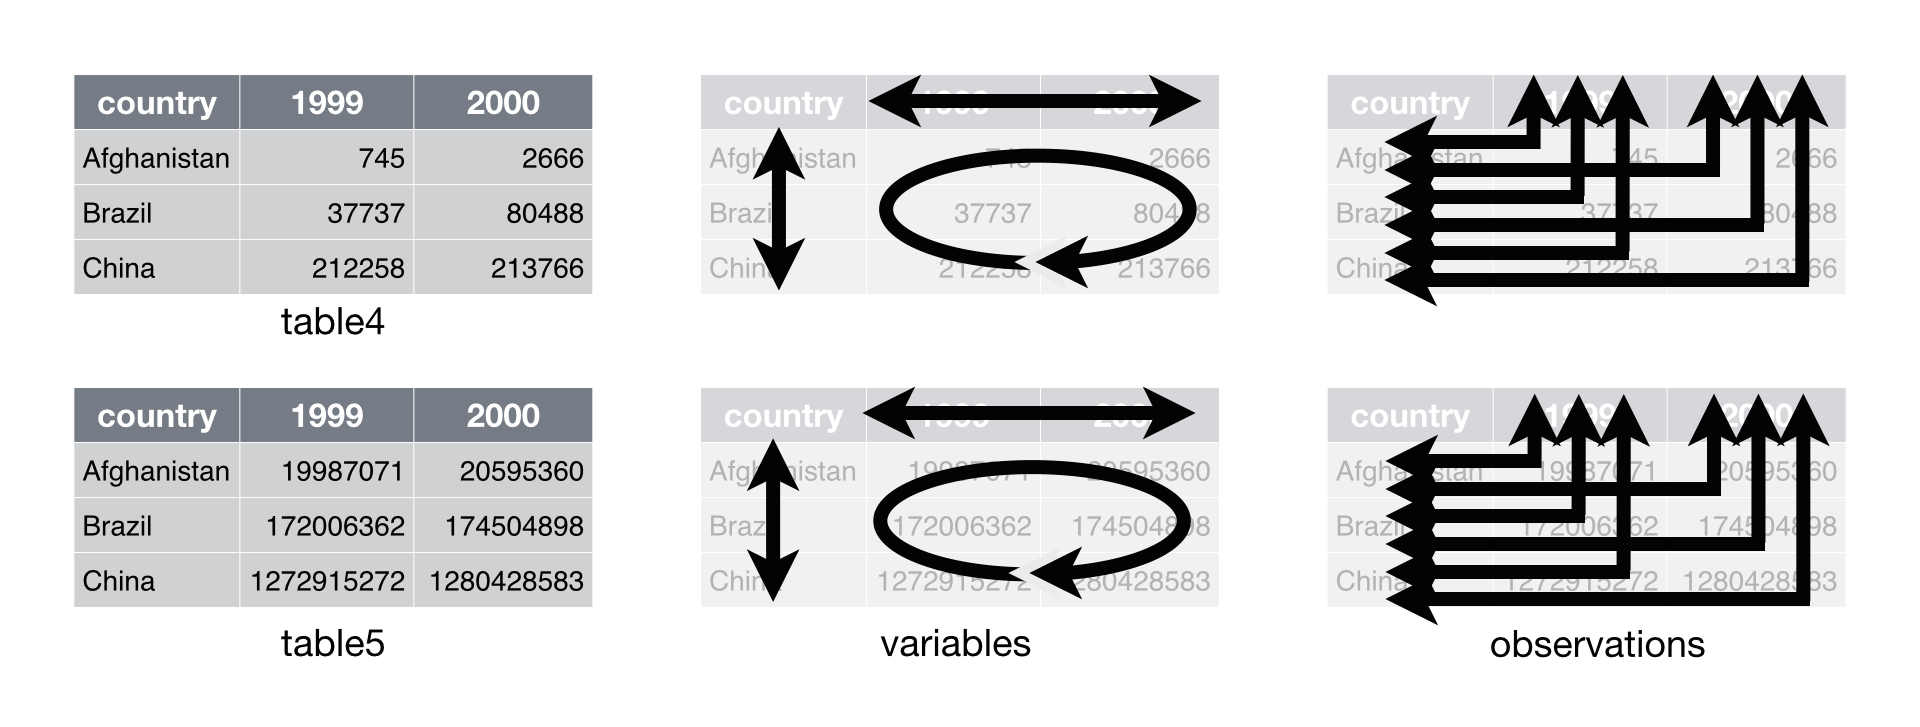
\includegraphics[width=1.1\linewidth]{tidy-7}
	
	\end{figure}
	
\end{frame}
%=============================================================================== %
\begin{frame}[fragile]
	\frametitle{Tidy Data with \texttt{R}}
	\Large
	\begin{itemize}
		\item The organization of data set four is inefficient in a second way as well. 
		\item Data set four separates the values of some variables across two separate tables. 
		\item This is inconvenient because you will need to extract information from two different places whenever you want to work with the data.
	\end{itemize}
\end{frame}
%=============================================================================== %
%\begin{frame}[fragile]
%	\frametitle{Tidy Data with \texttt{R}}
%	\Large
%	\begin{itemize}
%		\item 	 Compare this to data set one. With table1, you can use the same code to extract the values of year, \texttt{table1\$year}, that you use to extract the values of population.
%		\item To do so, you only need to change the name of the variable that you will access: \texttt{table1\$population}.
%	\end{itemize}
%	
%\end{frame}

%=============================================================================== %
%\begin{frame}[fragile]
%	\frametitle{Tidy Data with \texttt{R}}
%	\Large
%\begin{itemize}
%\item At this point, you might think that tidy data is so obvious that it is trivial. Surely, most data sets come in a tidy format, right? Wrong. 
%\item In practice, raw data is rarely tidy and is much harder to work with as a result. 
%\item Section 2.4 provides a realistic example of data collected in the wild.
%\end{itemize}
%
%\end{frame}
%=============================================================================== %
%\begin{frame}[fragile]
%	\frametitle{Tidy Data with \texttt{R}}
%	\Large
%\begin{itemize}
%\item Tidy data works well with R because R is a vectorized programming language. 
%\item Data structures in R are built from vectors and R’s operations are optimized to work with vectors. 
%\item Tidy data takes advantage of both of these traits.
%
%\item R stores tabular data as a data frame, a list of atomic vectors arranged to look like a table. Each column in the table is an atomic vector in the list.
%\end{itemize}
%
%\end{frame}

%=============================================================================== %
%\begin{frame}[fragile]
%	\frametitle{Tidy Data with \texttt{R}}
%	\Large
%Tidy data arranges values so that the relationships in the data parallel the structure of the data frame. Recall that each data set is a collection of values associated with a variable and an observation. In tidy data, each variable is assigned to its own column, i.e., its own vector in the data frame. As a result, you can extract easily the values of a variable in a tidy data set with R’s list syntax,
%\end{frame}
%=============================================================================== %
%\begin{frame}[fragile]
%	\frametitle{Tidy Data with \texttt{R}}
%	\Large
%\begin{verbatim}
%table1$cases
%
%## [1]    745   2666  37737  80488 212258 213766
%\end{verbatim}
%\end{frame}
%%=============================================================================== %
%\begin{frame}[fragile]
%\frametitle{Tidy Data with \texttt{R}}
%\Large
%\begin{itemize}
%\item R will return the values as an atomic vector, one of the most versatile data structures in R.
%
%\item  Many functions in R are written to take atomic vectors as input, as are R’s mathematical operators. 
%\item This adds up to an easy user experience; you can extract and manipulate the values of variables in tidy data with concise, simple code, e.g.,
%\end{itemize}
%
%\end{frame}
%=============================================================================== %
%\begin{frame}[fragile]
%\frametitle{Tidy Data with \texttt{R}}
%\Large
%\begin{verbatim}
%mean(table1$cases)
%
%## [1] 91276.67
%
%table1$cases / table1$population * 10000
%
%## [1] 0.372741 1.294466 2.193930 4.612363 1.667495 1.669488
%\end{verbatim}
%\end{frame}
%=============================================================================== %
%\begin{frame}[fragile]
%	\frametitle{Tidy Data with \texttt{R}}
%	\Large
%\begin{itemize}
%\item 	Tidy data also takes advantage of R’s vectorized operations. 
%\item In R, it is common to supply one or more vectors of values to a function or mathematical operator as input, and to receive a vector of values as output. 
%\end{itemize}
%
%\end{frame}
%=============================================================================== %
%\begin{frame}[fragile]
%	\frametitle{Tidy Data with \texttt{R}}
%	\Large
%\begin{itemize}
%\item To create the output, R applies the function in element-wise fashion: R first applies the function (or operation) to the first elements of each vector involved. \item Then R applies the function (or operation) to the second elements of each vector involved, and so on until R reaches the end of the vectors. 
%\item If one vector is shorter than the others, R will recycle its values as needed (according to a set of recycling rules).
%\end{itemize}	
%
%\end{frame}

%=============================================================================== %
%\begin{frame}[fragile]
%	\frametitle{Tidy Data with \texttt{R}}
%	\Large
%\begin{itemize}
%\item If your data is tidy, element-wise execution will ensure that observations are preserved across functions and operations. Each value will only be paired with other values that appear in the same row of the data frame.
%
%\item Do these small advantages matter in the long run? Yes. Consider what it would be like to do a simple calculation with each of the data sets from the start of the section.
%\end{itemize}
%
%\end{frame}

%%=============================================================================== %
%\begin{frame}[fragile]
%	\frametitle{Tidy Data with \texttt{R}}
%	\Large
%	
%If you use basic R syntax, your calculations will look like the code below. If you’d like to brush up on basic R syntax, see Appendix A: Getting Started.
%
%\end{frame}



%=============================================================================== %
%\begin{frame}[fragile]
%\frametitle{Tidy Data with \texttt{R}}
%\Large
%After you collect your input, you can calculate the rate.
%
%\begin{framed}
%\begin{verbatim}
%# Data set four
%cases <- c(table4$1999, table4$2000, table4$2001) 
%population <- c(table5$1999, table5$2000, table5$2001)
%cases / population * 10000
%\end{verbatim}
%\end{framed}
%
%\end{frame}
%%=============================================================================== %
%\begin{frame}[fragile]
%\frametitle{Tidy Data with \texttt{R}}
%\Large
%\begin{itemize}
%\item Data set one is much easier to work with than with data sets two, three, or four.
%\item To work with data sets two, three, and four, you need to take extra steps, which makes your code harder to write, harder to understand, and harder to debug.
%\end{itemize}
%
%\end{frame}
%%=============================================================================== %
%\begin{frame}[fragile]
%	\frametitle{Tidy Data with \texttt{R}}
%	\Large
%\begin{itemize}
%\item Keep in mind that this is a trivial calculation with a trivial data set. 
%\item The energy you must expend to manage a poor layout will increase with the size of your data. 
%\item Extra steps will accumulate over the course of an analysis and allow errors to creep into your work.
%\item You can avoid these difficulties by converting your data into a tidy format at the start of your analysis.
%\end{itemize}

\end{document}